\chapter{Funktionale Anforderungen}

%\section{Systemkontext}

\section{Systemfunktionen}

\newcounter{pfc}\setcounter{pfc}{10}

\begin{description}[leftmargin=5em, style=sameline]
	
	\begin{lhp}{pfc}{LF}{funk:spielverw}
		\item [Name:] Spielverwaltung
		\item [Beschreibung:] Das System verwaltet das von mehreren Spielern geteiltes Spiel in einem Spielraum. Das Spiel erfolgt nach den Spielregeln.
	\end{lhp}
	
	\begin{lhp}{pfc}{LF}{funk:zugriff}
		\item [Name:] Zugriffsverwaltung
		\item [Beschreibung:] Das System verwaltet den Zugang zum Spiel anhand Benutzerdaten. Spieler können sich registrieren, anmelden, abmelden sowie ihre Kontos löschen.
	\end{lhp}

	\begin{lhp}{pfc}{LF}{funk:spielraum}
		\item [Name:] Verwaltung der Spielräume
		\item [Beschreibung:] Das System verwaltet die Erstellung, Änderung und Löschung der Spielräume.
	\end{lhp}
	
	\begin{lhp}{pfc}{LF}{funk:bestenliste}
		\item [Name:] Bestenliste
		\item [Beschreibung:] Die Anzahl der gewonnen Spiele aller Spieler anzeigen.
	\end{lhp}
	
	\begin{lhp}{pfc}{LF}{funk:bots}
		\item [Name:] Intelligente Bots
		\item [Beschreibung:] Diese Bots ermöglichen erfahreneren Spielern, gegen einen vergleichbar starken Gegner anzutreten.
	\end{lhp}
	
	\begin{lhp}{pfc}{LF}{funk:chat}
		\item [Name:] Chat
		\item [Beschreibung:] Ein Dialogfenster ermöglicht den Spielern, ihre Angebote in der Tauschphase zu übermitteln und abzuschließen.
	\end{lhp}

\end{description}

% Gehört nicht in das Lastenheft.
%\section{Systemgrenze (Use Case Diagramm)}
%
%Die Systemgrenze wird auf der Abbildung~\ref{fig:systemgrenze} dargestellt\footnote{Weitere Erklärungen und Spezifizierungen, die sich auf Abgrenzungen der Verantwortlichkeiten vom System und weiteren Akteuren/Systemen können hier spezifiziert werden.}. 
%
%\begin{figure}
%\centering	
%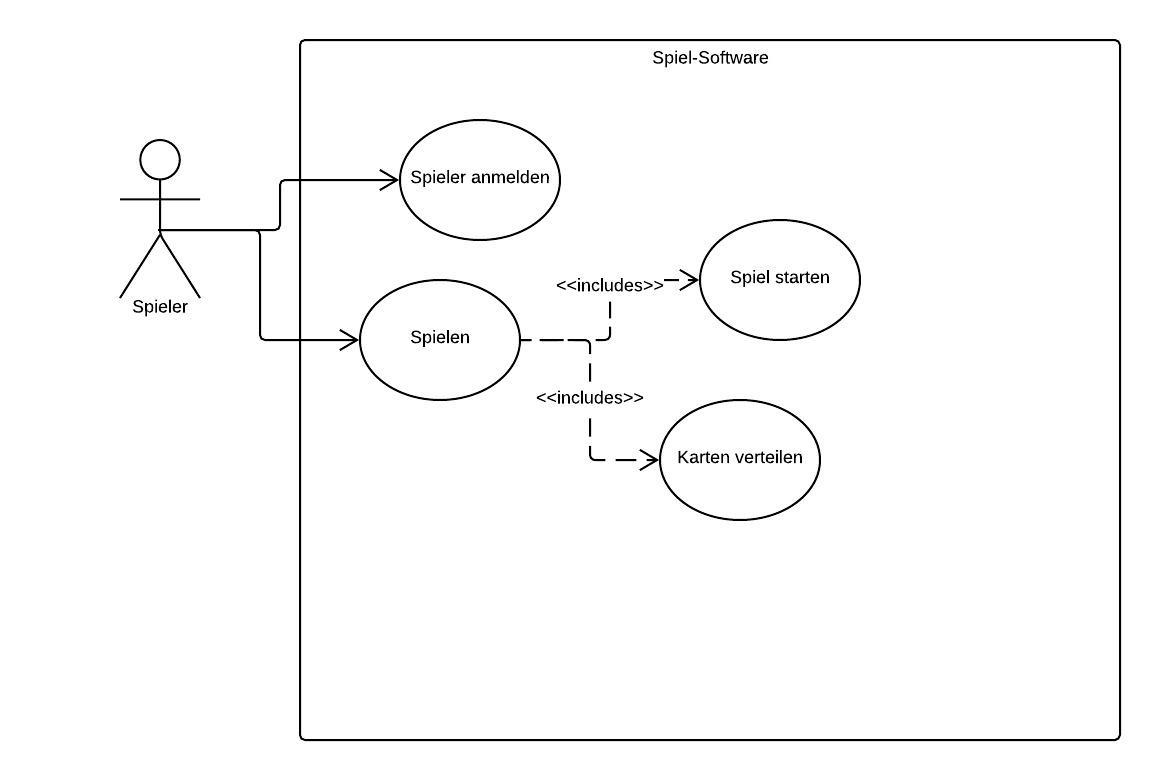
\includegraphics[width=0.9\textwidth]{img/ucd.jpg}
%\label{fig:systemgrenze}
%\caption{Ein Beispiel für Systemgrenzediagramm (Use Case Diagramm), das vor Abgabe anzupassen ist.}
%\end{figure}


